\documentclass[border=10pt]{standalone}
\usepackage{pgfplots}
\usepgfplotslibrary{colormaps}
\pgfplotsset{trig format plots=rad}
\begin{document}
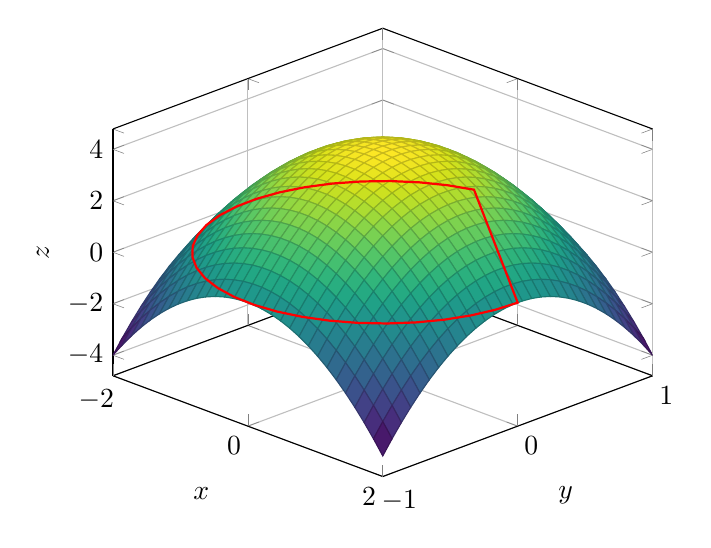
\begin{tikzpicture}
\begin{axis}[
    view={45}{30},
    xlabel=$x$, ylabel=$y$, zlabel=$z$,
    colormap/viridis,
    grid=major,
    samples=30
]
    % We want to plot the surface y = 4 - x^2 - 4z^2.
    % In PGFPlots, we can use \addplot3[surf] to plot z = f(x,y).
    % Here we have y = f(x,z). We can map (x,y,z) to (x,z,y) for the plotting.
    % Let X = x, Y = z, Z = y.
    % Then Z = 4 - X^2 - 4*Y^2.
    \addplot3[surf, domain=-2:2, y domain=-1:1] {4 - x^2 - 4*y^2};
    
    % Intersection ellipse at y=0 (Z=0 in our mapped coords)
    \addplot3[color=red, thick, domain=0:2*pi] ({2*cos(deg(x))}, {sin(deg(x))}, {0});
\end{axis}
\end{tikzpicture}
\end{document}
